\chapter{Evaluation}
\label{sec:eval}

We evaluated the performance of various application benchmarks
on a VM running on \rustsec{}, SeKVM, and mainline KVM.
We also tested the same
benchmarks on bare metal environment performances to establish a baseline
reference of the benchmark results. We ran the workloads on the Raspberry
Pi 4 model B development board, with a Broadcom BCM2711, quad-core
Cortex-A72 (ARM v8) 64-bit SoC at 1.5GHz, 4GB of RAM, and a 1 GbE NIC device.

\rustsec{}, SeKVM, and the mainline KVM are based on Linux 5.15.
QEMU v4.0.0 was used to start the virtual machines on Ubuntu 20.04. The guest
kernels also used Linux 5.15, and all kernels tested employed the same 
configuration. We requested the authors of~\cite{hypsec} and got a patch for
the Linux guest kernel to enable virtio.
\code{rustc} version 1.68.0-nightly was used to compile \rustcore{},
while clang 15.0.0 was used to compile the remaining components of
\rustsec{}, SeKVM, and the mainline KVM.

We configured the hardware with 2 physical CPUs and 1 GB of RAM for the bare
metal setup. Each VM that equips with 2 virtual CPUs for the VM setup, and 1
GB of RAM runs on the full hardware available.

We ran the benchmarks listed in \autoref{tab:benchmark} in the VMs on both
\rustsec{} and the mainline KVM. \autoref{fig:eval} shows the normalized
results. We normalized the results to bare-metal performance. 1.00 refers
to no virtualization overhead.
A higher value means higher overhead. The performance on real application
workloads show modest overhead overall for \rustsec{} compared to SeKVM and
mainline KVM.
The bare-metal setup actually performed worst in the \code{TCP\_MAERTS}
benchmark, this is caused by all four experimental setups saturated the 1GbE
NIC on the Raspberry Pi 4 model B, and also system noise was more significant
while measuring the bare-metal setup.
Benchmarks ran in the three VM setups resulted in at most 20\% difference,
we believe the differences are caused by various system noise factors e.g.
caches, kernel thread wakeups, and dynamic voltage frequency scaling.

\begin{table}
\centering
\footnotesize
\begin{tabular}{ |p{0.2\linewidth}|p{0.7\linewidth}| }
 \hline
 \small{\textbf{Name}} & \small{\textbf{Description}} \\
 \hline
 \small{Kernbench} & \small{Compilation of the Linux 6.0 kernel using \code{tinyconfig} for Arm with GCC 9.4.0.} \\
 \hline
 \small{Hackbench} & \small{\code{hackbench}~\cite{hackbench} using Unix domain sockets and 50 process groups running in 50 loops.} \\
 \hline
 \small{Netperf} & \small{\code{netperf}~\cite{netperf} v2.6.0 running the netserver on the server and the client with its default parameters in three modes: TCP\_STREAM (throughput), TCP\_MAERTS (throughput), and TCP\_RR (latency).} \\
 \hline
 \small{Apache} & \small{\code{Apache} v2.4.41 Web server running \code{ApacheBench}~\cite{ab} v2.3 on the remote client, which measures the number of handled requests per second when serving the 41 KB index.html file of the GCC 4.4 manual using 100 concurrent requests.} \\
 \hline
 \small{Memcached} & \small{\code{memcached} v1.5.22 using the \code{memtier}~\cite{memtier} benchmark v1.2.3 with its default parameters.} \\
 \hline
 \small{YCSB-Redis} & \small{\code{redis} v7.0.11 using the \code{YCSB}~\cite{YCSB} benchmark v0.17.0 with its default parameters.} \\
 \hline
\end{tabular}
\vspace{0.3cm}
\caption{Application Benchmarks}
\label{tab:benchmark}
\end{table}

\begin{figure}[hbtp]
    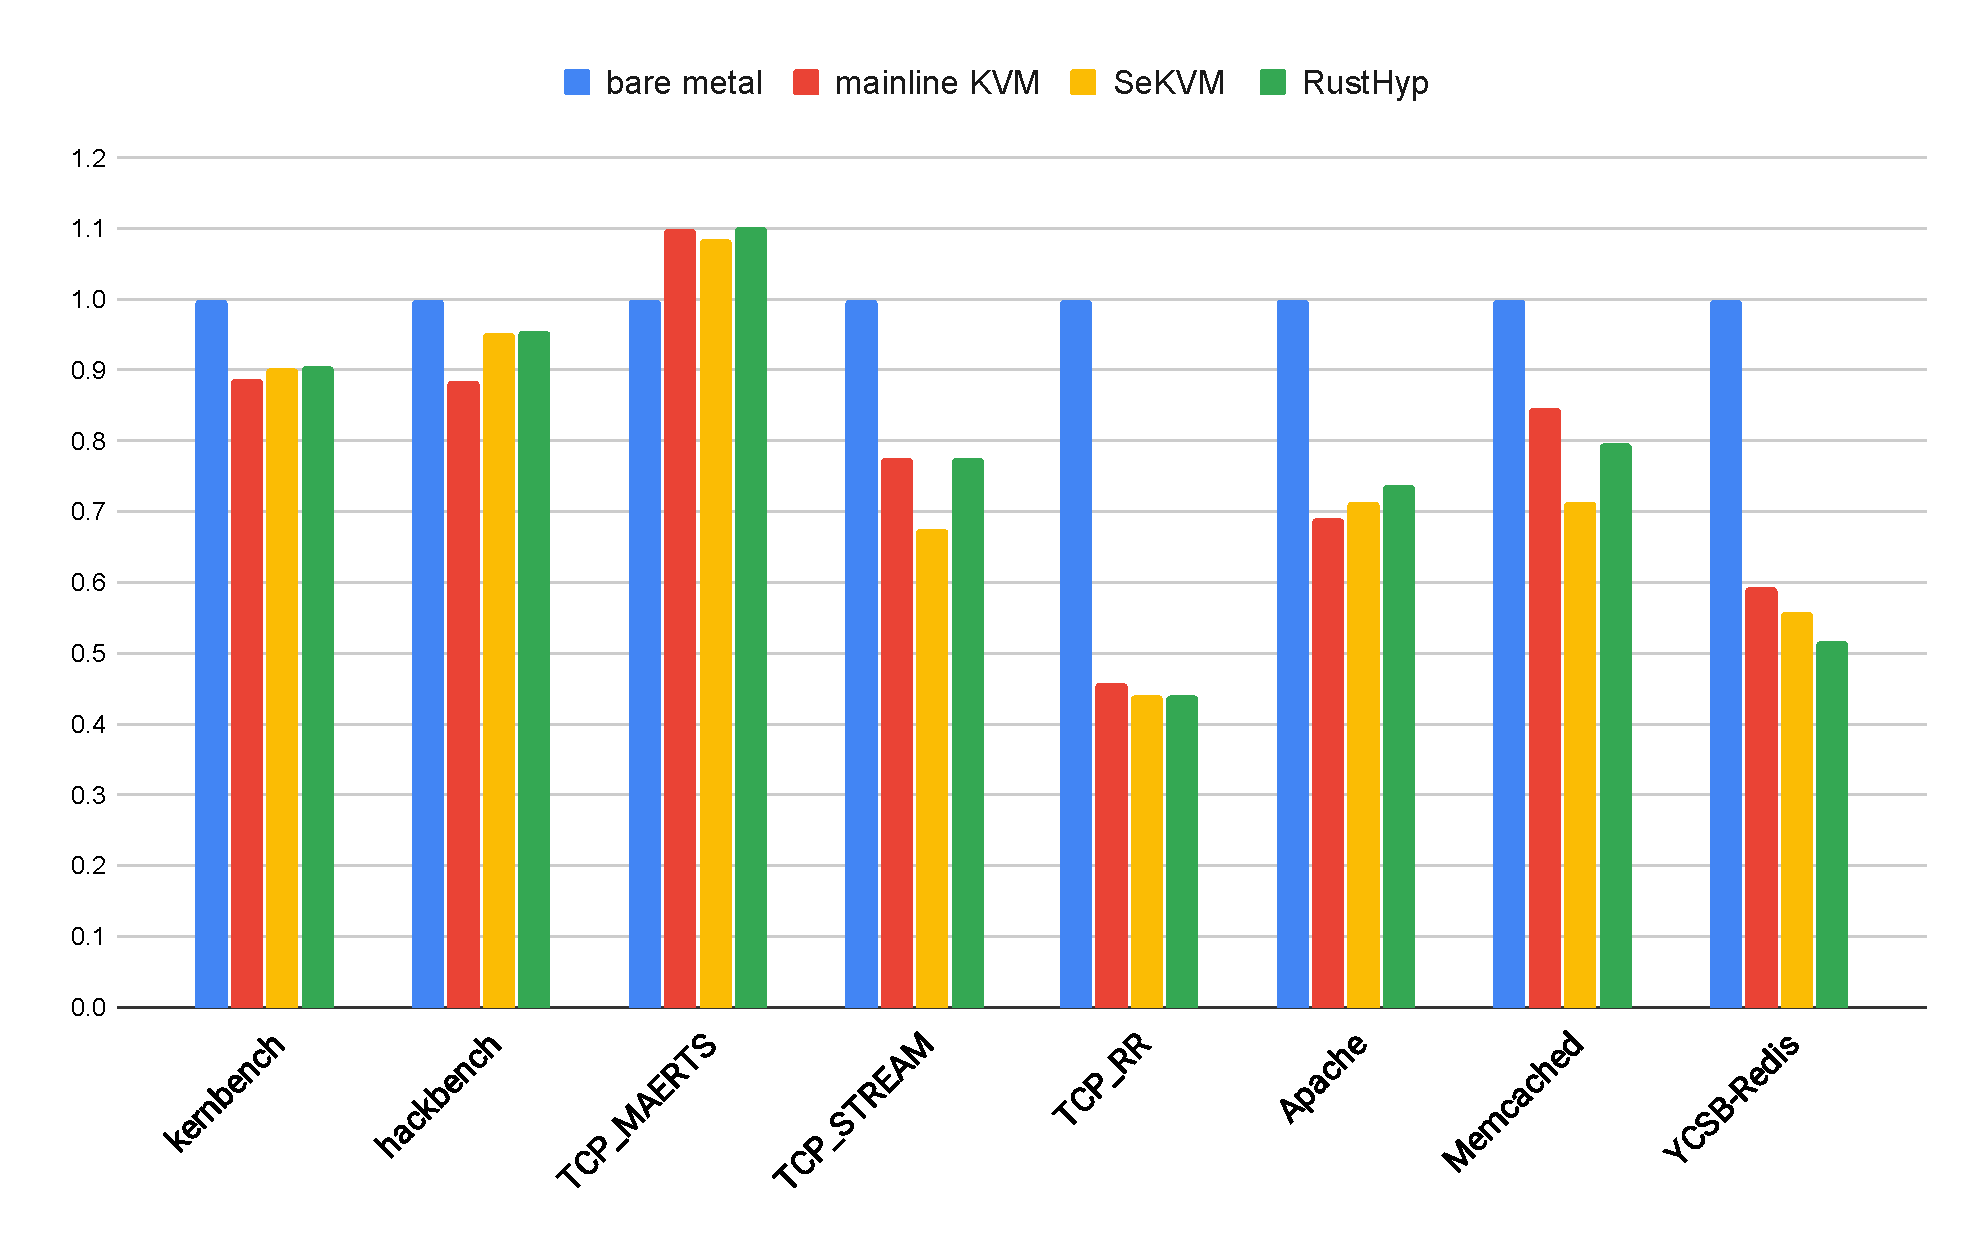
\includegraphics[scale=0.45]{figures/eval.pdf}
    \caption{Application Benchmark Performance}
    \label{fig:eval}
\end{figure}

